\documentclass[12pt]{report}

\usepackage{geometry}
\usepackage{fontspec}
\usepackage{xcolor}
\usepackage{colortbl}
\usepackage{tabularx}
\usepackage{tabularray}
\UseTblrLibrary{booktabs}
\usepackage{amstex}
\usepackage{amsmath}
\usepackage{tcolorbox}
\usepackage{titlesec}
\usepackage{setspace}
\usepackage[greek]{babel}
\usepackage{indentfirst}
\usepackage{fancyhdr}
%\usepackage[fontsize=13pt]{fontsize}

\geometry{a4paper, total={170mm,260mm}, left=20mm, top=20mm}

\setmainfont{Conduit ITC Hel Light}
\newfontfamily\fontDin{CF Din Condensed}
\newenvironment{Din}{\fontDin}{\par}
\newfontfamily\fontDinLight{CF Din Light Condensed}
\newenvironment{Din Light}{\fontDinLight}{\par}
\newfontfamily\fontDinMedium{CF Din Medium Condensed}
\newenvironment{Din Medium}{\fontDinMedium}{\par}
\newfontfamily\fontCode{Courier New}
\newenvironment{Code}{\fontCode}{\par}
\newfontfamily\fontTimes{Times New Roman}
\newenvironment{Times}{\fontTimes}{\par}

\newfontfamily\headingfont[]{CF Din Medium Condensed}

\addto\captionsgreek{% Replace "english" with the language you use
  \renewcommand{\contentsname}%
    {ΠΕΡΙΕΧΟΜΕΝΑ}%
}

\newtcolorbox{headerdark}{colback=darkgray, boxrule=0pt,arc=0pt, boxsep=12pt,left=2pt,right=2pt,leftrule=0pt}
\newtcolorbox{headerlight}{colback=gray!50, boxrule=0pt,arc=0pt, boxsep=2pt,left=2pt,right=2pt,leftrule=0pt}
\newtcolorbox{graycomment}{colback=gray!25, boxrule=0pt,arc=0pt, boxsep=2pt,left=2pt,right=2pt,leftrule=1pt, grow to left by=-28pt,  grow to right by=-28pt}

% Το στιλ των νέων κεφαλαίων/sectionσ
\titleformat{\chapter}[block]
    {\color{black} \fontDinLight \large } % global formatting (number and title)
    {\color{white} \fontDin \colorbox{black!80} {\hspace{7pt}\thechapter\hspace{7pt}}} % label: number and its formatting
    {} % spacing between number and title
    {\colorbox{gray!25}} % optional (content between number and title)

\titleformat{\section}[block]
    {\color{black} \fontDinLight \large} % global formatting (number and title)
    {\color{white} \fontDin \colorbox{black!80} {\hspace{5pt}\thesection\hspace{5pt}}} % label: number and its formatting
    {} % spacing between number and title
    {\colorbox{gray!25}} % optional (content between number and title)

\titlespacing*{\chapter}
   {0pt}{0}{0.4em}  % left before after

\titlespacing*{\section}
   {0pt}{1em}{0.4em}  % left before after

\titleclass{\chapter}{straight}


%% Setting for the column separator
%\colorlet{shadecol}{black!20}
%\setlength\columnsep{12pt}
%\makeatletter   % This change vertical bar to a dotted line
%\newcommand{\latexcolumnseprulecolor}{\color{shadecol}}
%\renewcommand\dotfill[1][0.4em]{%
%  \leavevmode\cleaders\hb@xt@ #1{\hss .\hss}\hfill\kern\z@}
%\patchcmd{\@outputdblcol}%
%  {\vrule\@width\columnseprule}%
%  {\rotatebox{90}{\parbox{\textheight}{\dotfill[0.3em]}}}%
%  {}{}
%\makeatother
%
%% Command to render shaded heading
%\newsavebox\labbox
%\NewDocumentCommand\shadedsec{O{1.5\baselineskip} O{0.33\dimexpr#1} m}{%
%  \sbox\labbox{%
%    \colorbox{black!80}{%
%      \textcolor{white}{\hspace{0.5em}#3\hspace{0.5em}}}}
%  \addvspace{#1}
%  \noindent%
%  \nopagebreak%
%  \usebox\labbox
%  {\color{shadecol}\rule[-\fboxsep]{\dimexpr\columnwidth-\wd\labbox}{\dimexpr\ht\labbox+\fboxsep}}%
%  \vspace{#2}\par}


% Ρύθμση αλλαγής γραμμής
\tolerance=1
\emergencystretch=\maxdimen
\hyphenpenalty=10000 % Για να μην κάνει συλλαβισμό στις λέξεις
\hbadness=10000

% Αλλαγή απόστασης μεταξύ παραγράφων
\setlength{\parskip}{6pt}

% Ρύθμιση Headers/Footers
\pagestyle{fancy}
\renewcommand{\headrulewidth}{0pt}
\fancyhead{}\fancyfoot{}
\fancyhead[R]{\fontDinLight ΑΛΕΞΑΝΔΡΟΣ ΞΙΑΡΧΟΣ \(\cdot\) 1059619\hspace{10pt}\colorbox{black!50}{\color{white}\fontDin\thepage}}

% Συνεχόμενη αρίθμηση ανά chapters
\counterwithout{footnote}{chapter}

\endinput


\begin{document}

    \begin{titlepage}
        \centering

        \renewcommand{\arraystretch}{1.1} % Increase row height
        \begin{tabularx}{\textwidth}{@{}m{0.9\textwidth}X@{}}
            \centering \raggedleft \cellcolor{lightgray!25} Αλέξανδρος Ξιάρχος\\ {\footnotesize st1059619@ceid.upatras.gr} & \centering\cellcolor{darkgray}\fontDin \raisebox{-1pt}{\color{white}1059619 \\}
        \end{tabularx}

        \vspace*{12em}
        \begin{headerlight}
            \begin{Din}
                \centering
                {ΠΑΝΕΠΙΣΤΗΜΙΟ ΠΑΤΡΩΝ \(\cdot\) ΤΜΗΜΑ ΜΗΧΑΝΙΚΩΝ Η/Υ ΚΑΙ ΠΛΗΡΟΦΟΡΙΚΗΣ}
            \end{Din}
        \end{headerlight}

        \begin{headerdark}
            \begin{Din Medium}
                \centering
                \huge \textcolor{white}{ΑΝΑΚΤΗΣΗ ΠΛΗΡΟΦΟΡΙΑΣ}
            \end{Din Medium}
        \end{headerdark}

        \begin{headerlight}
            \begin{Din}
                \centering
                ΕΡΓΑΣΤΗΡΙΑΚΗ ΑΣΚΗΣΗ \(\cdot\) 2023 \(\textendash\) 2024
            \end{Din}
        \end{headerlight}

        \vspace*{10em}

    \end{titlepage}

    \tableofcontents
    \pagebreak

%   ===================================================================================================================


    \chapter{ΕΙΣΑΓΩΓΗ}


    \section{ΕΠΙΛΟΓΗ ΣΥΣΤΗΜΑΤΩΝ ΣΤΑΘΜΙΣΗΣ TF-IDF}
    Καταρχάς πρέπει να επιλέξουμε τα δύο συστήματα στάθμισης των βαρών για τα διανύσματα που θα χρησιμοποιήσουμε.

    \subsection{ΠΡΩΤΟ ΣΥΣΤΗΜΑ ΣΤΑΘΜΙΣΗΣ}
    Το πρώτο σύστημα στάθμισης θα είναι μια παραλλαγή\footnote{Το σύστημα αναφέρεται ως παραλλαγή των Salton-Buckley για το λόγο ότι δεν έχει συμπεριληφθεί κάποιος παράγοντας κανονικοποίσης, μιας και τα έγγραφα είναι \textit{περίπου} ισομεγέθη (μέσος όρος 350 λέξεις).} του προτεινόμενου ως καλύτερου πλήρως σταθμισμένου συστήματος σύμφωνα με τους Salton-Buckley\footnote{Gerard Salton, Christopher Buckley, Term-weighting approaches in automatic text retrieval, Information Processing \& Management, Volume 24, Issue 5, 1988, Pages 513-523, ISSN 0306-4573}
    {\fontTimes (best fully weighted system)}. \linebreak Θα χρησιμοποιήσουμε την \textbf{απλή συχνότητα εμφάνισης} {\fontTimes (raw term frequency)} για το TF βάρος των εγγράφων,
    \[ \text{\textbf{Σύστημα \#1:}\hspace{5pt}TF}_{\scriptsize \text{εγγράφων}}=\hspace{5pt} f_{i,j} \]
    όπου \(f_{ij}\) οι φορές που ο όρος εμφανίζεται σε ένα έγγραφο, τη \textbf{διπλή 0,5 κανονικοποίηση} για το TF βάρος των ερωτημάτων {\fontTimes(augmented normalized TF)},
    \[ \text{\textbf{Σύστημα \#1:}\hspace{5pt}TF}_{\scriptsize \text{ερωτημάτων}}=\hspace{5pt} 0.5 + 0.5 \frac{f_{i,j}}{max_i\hspace{3pt}f_{i,j}} \]
    και τέλος την \textbf{απλή ανάστροφη συχνότητα εμφάνισης} για το IDF βάρος και των εγγράφων και των ερωτημάτων:
    \[\text{\textbf{Σύστημα \#1:}\hspace{5pt}IDF}_{\scriptsize\begin{matrix}
                                                                  \text{εγγράφων}\\\text{ερωτημάτων}
    \end{matrix}}=\hspace{5pt} \log{\frac{N}{n_i}} \]
    όπου \(N\) το πλήθος των εγγράφων και \(n_i\) ο αριθμός των εγγράφων στα οποία εμπεριέχεται ο όρος.

    \subsection{ΔΕΥΤΕΡΟ ΣΥΣΤΗΜΑ ΣΤΑΘΜΙΣΗΣ}
    Ως δεύτερο σύστημα στάθμισης θα χρησιμοποιήσουμε το καλύτερα σταθμισμένο πιθανολογικό σύστημα σύμφωνα με τους Salton-Buckley\footnotemark[1]
    {\fontTimes (best weighted probabilistic weight)} με
    \[ \text{\textbf{Σύστημα \#2:}\hspace{5pt}βάρος όρου}_{\scriptsize \text{εγγράφων}}=\hspace{5pt} 0.5 + 0.5 \frac{f_{i,j}}{max_i\hspace{3pt}f_{i,j}}\]
    \[ \text{\textbf{Σύστημα \#2:}\hspace{5pt}βάρος όρου}_{\scriptsize \text{ερωτημάτων}}=\hspace{5pt} \log{\frac{N - n_i}{n_i}}. \]

    Και τα δύο αυτά συστήματα στάθμισης έχουν επιφέρει τα ακριβέστερα αποτελέσματα και στο σύνολο των συλλογών στα οποία έχουν εξεταστεί
    αλλά και ειδικότερα σε ιατρικές {\fontTimes (MED)} συλλογές. Επομένως, συνολικά έχουμε:

    \noindent
    \begin{tblr}{
        colspec={>{\centering\arraybackslash}m{3.5cm}>{\centering\arraybackslash}m{6.1cm}>{\centering\arraybackslash}m{6.1cm}},
        row{2}={bg=lightgray!50}, row{3}={bg=lightgray}, row{1}={bg=black!90,fg=white}}
        Σύστημα στάθμισης & Βάρος όρου εγγράφου                                     & Βάρος όρου ερωτήματος                                                                \\
        1                 & \[f_{i,j} \times \log{\frac{N}{n_i}} \]                 & \[(0.5 + 0.5 \frac{f_{i,j}}{max_i\hspace{3pt}f_{i,j}}) \times \log{\frac{N}{n_i}} \] \\
        2                 & \[0.5 + 0.5 \frac{f_{i,j}}{max_i\hspace{3pt}f_{i,j}} \] & \[\log{\frac{N - n_i}{n_i}} \]                                                       \\
    \end{tblr}
    \\\\


%   ===================================================================================================================


    \chapter{ΥΛΟΠΟΙΗΣΗ ΜΟΝΤΕΛΩΝ}
    Η εργασία υλοποιήθηκε σε Python χρησιμοποιώντας τις βιβλιοθήκες:

    \begin{tblr}{
        colspec={>{\centering\arraybackslash}m{5cm}>{\centering\arraybackslash}m{10cm}},
        row{2,4,6,8}={bg=lightgray!50}, row{3,5,7,9}={bg=lightgray}, row{1}={bg=black!90,fg=white}}
        Βιβλιοθήκη                   & Περιγραφή                          \\
        \textbf{\texttt{os}}         & σύνδεση με λειτουργικό σύστημα     \\
        \textbf{\texttt{json}}       & αποθήκευση-ανάγνωση JSON αρχείων   \\
        \textbf{\texttt{nltk}}       & αφαίρεση stopwords, stemming       \\
        \textbf{\texttt{numpy}}      & υπολογισμός ομοιότητας συνημιτόνου \\
        \textbf{\texttt{math}}       & υπολογισμός λογαρίθμων             \\
        \textbf{\texttt{matplotlib}} & γραφικές παραστάσεις               \\
    \end{tblr}

    Αυτή είναι η δομή των αρχείων κώδικα όπου έχει χωριστεί η υλοποίηση: \\
    \begin{minipage}{.5\textwidth}
        \centering
        \begin{forest}
            for tree={
                font=\tt,
                grow'=00,
                child anchor=west,
                parent anchor=south,
                anchor=west,
                calign=first,
                edge path={
                    \noexpand\path [draw, \forestoption{edge}]
                    (!u.south west) +(7.5pt,0) |- node[fill,inner sep=1.5pt] {} (.child anchor)\forestoption{edge label};
                },
                before typesetting nodes={
                    if n=1
                        {insert before={[,phantom]}}
                        {}
                },
                fit=band,
                before computing xy={l=15pt},
            }
            [src
            [main.py]
            [tools.py]
            [preprocessing.py]
            [inverted\_index.py]
            [vector\_space\_model.py]
            ]
        \end{forest}
    \end{minipage}%
    \begin{minipage}{.5\textwidth}
        \centering
        \begin{forest}
            for tree={
                font=\tt,
                grow'=00,
                child anchor=west,
                parent anchor=south,
                anchor=west,
                calign=first,
                edge path={
                    \noexpand\path [draw, \forestoption{edge}]
                    (!u.south west) +(7.5pt,0) |- node[fill,inner sep=1.5pt] {} (.child anchor)\forestoption{edge label};
                },
                before typesetting nodes={
                    if n=1
                        {insert before={[,phantom]}}
                        {}
                },
                fit=band,
                before computing xy={l=15pt},
            }
            [src
            [colBERT\_preprocessing.py]
            [colBERT.ipynb]
            [evaluation\_metrics.py]
            ]
        \end{forest}
    \end{minipage}%

    Τέλος, η υλοποίηση του colBERT μοντέλου έχει πραγματοποιηθεί στο Google Colab ως Juputer Notebook.


    \section{ΠΡΟΕΠΕΞΕΡΓΑΣΙΑ ΕΓΓΡΑΦΩΝ \& ΒΟΗΘΗΤΙΚΕΣ ΣΥΝΑΡΤΗΣΕΙΣ}

    \subsection{\tt tools.py}

    Το αρχείο \texttt{tools.py} περιλαμβάνει βοηθητικές συναρτήσεις για κάποιες επαναλαμβανόμενες διαδικασίες της υλοποίησης.

    Η συνάρτηση \texttt{\textbf{get\_docs}()}, χρησιμοποιώντας την \texttt{os} βιβλιοθήκη, διαβάζει το πλήθος των αρχείων της συλλογής.\footnote{Να σημειωθεί ότι το πλήθος των εγγράφων διαφέρει από την αύξουσα αρίθμησή τους. Συγκεκριμένα έχουμε 1209 έγγραφα αριθμημένα από το \texttt{000001} ως \texttt{01239}. Με άλλα λόγια υπάρχουν αριθμοί στη συλλογή που δεν αντιστοιχούν σε έγγραφα. Συνεπώς δεν θα μπορούσαμε να χρησιμοποιήσουμε κάποια αριθμητική επανάληψη, για παράδειγμα, για την εισαγωγή των εγγράφων.}
    Η συνάρτηση, αφού αφαιρέσει το escape character \texttt{'\textbackslash n'}, το οποίο προκύπτει από την μορφολογία των εγγράφων (η κάθε λέξη είναι τοποθετημένη σε διαφορετική γραμμή),
    δημιουργεί \linebreak και επιστρέφει μια λίστα από tuples, με κάθε tuple να αντιστοιχεί σε κάθε αρχείο-έγγραφο. \linebreak
    Έτσι τα έγγραφα έχουν τη δομή:
    \begin{graycomment}
        \centering
        \verb|doc = ('docID', ['λήμμα_1', 'λήμμα_2' ...])|
    \end{graycomment}

    \noindent όπου \texttt{docID} η αρίθμηση του κάθε εγγράφου και \verb|λήμμα_n| η κάθε λέξη-λήμμα του εγγράφου.
    Αυτός θα είναι ο τρόπος αποθήκευσης και προσπέλασης των εγγράφων σε όλη την υλοποίηση.

    Η συνάρτηση \texttt{strip()} της \verb|get_docs()| είναι απαραίτητη για την αφαίρεση των \texttt{\textbackslash n} χαρακτήρων
    που προκύπτουν από τη μορφολογία των εγγράφων (μιας και κάθε λέξη είναι σε νέα γραμμή).
    Με παρόμοιο τρόπο η συνάρτηση \texttt{\textbf{get\_queries}()} επιστρέφει τη λίστα με τα ερωτήματα της συλλογής,
    η \texttt{\textbf{get\_relevant}()} τη λίστα με τα σχετικά έγγραφα ανά ερώτημα και η \texttt{\textbf{get\_json\_file}()} τα περιεχόμενα ενός JSON αρχείου.

    \subsection{\tt preprocessing.py}

    Στο αρχείο \texttt{preprocessing.py}, και συγκεκριμένα στις συναρτήσεις \texttt{\textbf{preprocess\_collection}()} και \texttt{\textbf{preprocess\_queries}()}
    πραγματοποιείται η προεπεξεργασία των εγγράφων, συγκεκριμένα η αφαίρεση των stopwords και το stemming.

    Χρησιμοποιούμε τη \texttt{nltk} βιβλιοθήκη. Κάθε λέξη από τη συλλογή των εγγράφων αφού περάσουν από τον \texttt{PorterStemmer} της \texttt{nltk}
    και ελεγχθούν ότι δεν ανήκουν στη λίστα των stopwords, επιστρέφονται σε παρόμοια μορφή όπως δημιουργήθηκαν στη \verb|get_docs()|.
    Αντίστοιχη διαδικασία πραγματοποιείται και για την προεπεξεργασία των ερωτημάτων, στη \verb|preprocess_queries()|.


    \section{ΑΝΕΣΤΡΑΜΜΕΝΟ ΕΥΡΕΤΗΡΙΟ}

    Το ανεστραμμένο ευρετήριο δημιουργείται στη συνάρτηση \texttt{\textbf{create\_inverted\_index}()} του αρχείου \verb|inverted_index.py|.
    Τα έγγραφα, μετά την προεπεξεργασία τους, εισέρχονται σε μια δομή επανάληψης, \linebreak η οποία δημιουργεί το ανεστραμμένο ευρετήριο ως μορφή λεξικού ως εξής:

    \begin{graycomment}
        \centering
        \texttt{\small \textbf{inverted\_index['λήμμα']} = \\ \{('docID\(_\texttt{1}\)': <φορές εμφάνισης>), ('docID\(_\texttt{2}\)': <φορές εμφάνισης>), \(\ldots\) \}}
    \end{graycomment}

    Κάθε value του dictionary είναι ένα σύνολο\footnote{Έχει επιλεχθεί set για εξοικονόμιση μνήμης, μας και δεν μας ενδιαφέρει η σειρά των tuples.} το οποίο περιλαμβάνει ένα ή περισσότερα tuples με το \texttt{docID}
    και τη συχνότητα εμφάνισης του λήμματος στο συγκεκριμένο έγγραφο. Η συχνότητα υπολογίζεται μέσω της \texttt{count()} σε όλο το έγγραφο ανά λήμμα.

    Αυτό είναι ένα παράδειγμα του τελικού ανεστραμμένου ευρετηρίου:

    \begin{graycomment}
        \centering
        \texttt{\small \textbf{inverted\_index} = \{ \(\ldots\) 'coronari': \{('01217', 2), ('00779', 1)\}, \\ 'mobil': \{('00673', 2)\}, 'strain': \{('00179', 7)\}, \(\ldots\) \}}
    \end{graycomment}


    \section{ΥΛΟΠΟΙΗΣΗ VECTOR SPACE ΜΟΝΤΕΛΟΥ}

    Η υλοποίηση του Vector Space μοντέλου γίνεται στο αρχείο \verb|vector_space_model.py|.
    Η συνάρτηση \texttt{\textbf{run\_vsm}(doc\_collection, queries, inverted\_index)}, μέσω μιας επανάληψης ώστε να καλυφθούν όλα τα queries,
    καλεί την συνάρτηση \texttt{\textbf{vsm}(doc\_collection, query, inverted\_index, model\_type)}, όπου \texttt{model\_type = '1'} ή \texttt{'2'}, ανάλογα με το σύστημα στάθμισης που θέλουμε να χρησιμοποιήσουμε.

    H συνάρτηση \texttt{vsm()} αρχικά υπολογίζει τις συχνότητες \(f_{i,j}\) κάθε όρου του εκάστοτε ερωτήματος:
    \begin{graycomment}
        \texttt{query\_tfs\(_{\textit{\hspace{2pt}len(query)}}\)\ = \{ \(\ldots\) 'calcium': 1, 'effect': 2 \(\ldots\) \}}
    \end{graycomment}

    Στη συνέχεια διατρέχεται κάθε όρος από το ερώτημα \texttt{query}. Αν ο όρος του ερωτήματος υπάρχει στο ανεστραμμένο ευρετήριο, υπολογίζεται η IDF τιμή του.
    και στη συνέχεια το TF-IDF βάρος του ερωτήματος, όπου θα αποθηκευτεί στο λεξικό \verb|query_tfidfs|.

    \begin{graycomment}
        \texttt{\small query\_ifidf\(_{\textit{\tt\hspace{2pt}len(query)}}\)\ = \{ \(\ldots\) 'calcium': 3.6318, 'effect': 1.76483 \(\ldots\) \}}
    \end{graycomment}

    Στη συνέχεια, για κάθε όρο του ερωτήματος, διατρέχουμε όλα τα έγγραφα της συλλογής. Αν το έγγραφο περιλαμβάνει τον όρο του ερωτήματος που εξετάζουμε
    (κάτι που ελέγχουμε μέσω της \verb|docs_containing_term|), τότε μέσω του ανεστραμμένου ευρετηρίου, αποθηκεύεται η TF τιμή του, υπολογίζεται
    το TF-IDF βάρος του εγγράφου και αποθηκεύεται στο \verb|doc_tfidfs[docID]|. Αν το έγγραφο δεν περιλαμβάνει τον όρο, αποθηκεύουμε 0.

    \begin{graycomment}
        \texttt{\small doc\_ifidf\(_{\textit{\tt\hspace{2pt}len(doc\_collection)}}\)\ = \{'000001': [0, 0, 0.0, 1.76, 1.5]_{\textit{\tt len(query)}} \(\ldots\)\}}
    \end{graycomment}

    Η διαδικασία επαναλαμβάνεται για κάθε όρο του ερωτήματος. Επειδή τα δύο μοντέλα έχουν διαφορετικό σύστημα στάθμισης, ο υπολογισμός των βαρών βρίσκεται μέσα σε συνθήκες, ανάλογα με το \verb|model_type| που χρησιμοποιούμε.

    Το αποτέλεσμα είναι να έχουμε δημιουργήσει το διάνυσμα ερωτήματος και 1209 διανύσματα εγγράφων. Στην λίστα \texttt{similarity} υπολογίζουμε
    την ομοιότητα συνημιτόνου μεταξύ του διανύσματος ερωτήματος και κάθε διανύσματος εγγράφου. Επειδή κάποια διανύσματα αποτελούνται από μηδενικά,
    στους υπολογισμούς οδηγούμαστε σε \texttt{nan} τιμές, που μετατρέπουμε σε \texttt{0}. Η συνάρτηση εν τέλει επιστρέφει τα 100 κείμενα με την μεγαλύτερη ομοιότητα.


    \section{ΥΛΟΠΟΙΗΣΗ colBERT}

    Στο αρχείο \verb|colBERT_preprocessing.py| γίνεται η προεπεξεργασία των εγγράφων και ερωτημάτων ώστε να δοθούν ως inputs στο colBERT μοντέλο.
    Συγκεκριμένα γίνεται μετατροπή των ερωτημάτων σε κεφαλαία και αποθήκευση σε JSON αρχεία τα έγγραφα και ερωτήματα σε λεξικά ως εξής:

    \begin{graycomment}
        \texttt{\small colBERTdocs = \{"docID\(_\text{i}\)": "<doc\(_\text{i}\)>", \(\ldots\) \} \\}
        \texttt{\small colBERTqueries = \{"queryID\(_\text{i}\)": "<query\(_\text{i}\)>", \(\ldots\) \}}
    \end{graycomment}

    Η εκτέλεση του colBERT μοντέλου πραγματοποιείται μέσω του αρχείου \texttt{colBERT.ipynb} στο Google Colab.
    Τα λεξικά των JSON αρχείων αφού διαβαστούν, διασπώνται σε 2 ξεχωριστές λίστες: \verb|doc_list.keys()| για τα IDs, \verb|doc_list.values()| για το περιεχόμενο και αντίστοιχα για τα ερωτήματα.

    Μετά τη δημιουργία του Indexer και του Searcher με \verb|doc_maxlen = 300|, \verb|kmeans_niters = 20| και \verb|k = 100|,
    δημιουργείται μια λίστα τα 100 πιο σχετικά κείμενα, ο οποία γίνεται download ως JSON αρχείο.


    \chapter{ΜΕΤΡΙΚΕΣ ΑΞΙΟΛΟΓΗΣΗΣ}
    Μιας και ως δεδομένα έχουμε τα πραγματικά σχετικά έγγραφα (\verb|Relevant_20|), για την σύγκριση των μοντέλων χρησιμοποιήθηκαν:
    \begin{itemize}
        \item \textbf{Διάγραμμα ανάκλησης-ακρίβειας} {\fontTimes(Precision-Recall curve)}. Το διάγραμμα παρουσιάζει ενδιαφέρον γιατί \textendash συνδυάζοντας τις μετρικές ανάκλησης και ακρίβειας\textendash \hspace{1pt}
        παρουσιάζει με προφανή τρόπο τα σημεία που το μοντέλο παρουσιάζει μεγαλύτερη ακρίβεια και ταυτόχρονα λιγότερη ανάκληση και αντίστροφα.

        \begin{multicols}{2}
            \centering
            \( \text{Ακρίβεια} = \frac{\text{αριθμός σχετικών ανακτηθέντων κειμένων}}{\text{αριθμός εγγράφων που ανακτήθηκαν}} \) \\
            \( \text{Ανάκληση} = \frac{\text{αριθμός σχετικών ανακτηθέντων κειμένων}}{\text{αριθμός σχετικών εγγράφων στη συλλογή}} \)
        \end{multicols}

        \item \textbf{Μέσος Όρος Μέσης Ακρίβειας} {\fontTimes (Mean Average Precision \textendash\hspace{1pt} MAP)}. Χρησιμοποιούμε την συγκεκριμένη μετρική
        για τη δημιουργία μιας συνοπτικές ενιαίας τιμής της κατάταξης, χρησιμοποιώντας τα πολλαπλά ερωτήματα που έχουμε.
        \vspace{-10pt}
        \[ \text{Μέση Ακρίβεια} = \sum_{i=1}^{i=k}(\text{ανάκληση}[i] - \text{ανάκληση}[i-1])\times\text{ακρίβεια}[i] \]
        \vspace{-5pt}
        \[ \text{MAP} = \frac{\text{Μέση Ακρίβεια για κάθε ερώτημα}}{\text{Σύνολο ερωτημάτων}} \]
    \end{itemize}

    Η συνάρτηση \verb|recall_precision()| με εισόδους τα αποτελέσματα των μοντέλων και τα πραγματικά σχετικά έγγραφα,
    υπολογίζει τις τιμές ανάκλησης και ακρίβειας για κάθε ερώτημα και τις επιστρέφει σε μία λίστα. Η λίστα αυτή εισάγεται στην \verb|mean_average_precision()|
    όπου υπολογίζεται ο Μέσος Όρος Μέσης Ακρίβειας.


    \section{\hspace{1pt}ΑΠΟΤΕΛΕΣΜΑΤΑ\hspace{1pt}}

    Οι τιμές του Μέσου Όρου Μέσης Ακρίβειας (MAP) για τα τρία μοντέλα είναι:
    \begin{graycomment}
        \centering
        \begin{tabular}{ l l }
            \textbf{VSM #1}  & \texttt{0.016352} \\
            \textbf{VSM #2}  & \texttt{0.008598} \\
            \textbf{colBERT} & \texttt{0.007089}
        \end{tabular}
    \end{graycomment}

    Στα διαγράμματα ανάκλησης-ακρίβειας που παρουσιάζονται παρακάτω, παρατηρούμε πως σχεδόν πάντα το \textbf{VSM \#2} μοντέλο τερματίζει τελευταίο.
    Αυτό είναι κάτι που συνάδει με τα αποτελέσματα των Salton-Buckley, αλλά είναι και λογικό αν λάβουμε υπόψη τον τρόπο υπολογισμού των βαρών του, στα οποία δεν εμπεριέχεται ο παράγοντας IDF στα βάρη των εγγράφων.

    Από την άλλη, ξεκάθαρη υπεροχή παρουσιάζει το \textbf{VSM \#1} μοντέλο και σε ακρίβεια αλλά και σε ανάκληση, κάτι που είναι εξίσου σημαντικό όταν έχουμε να κάνουμε με επιστημονικές/ιατρικές αναζητήσεις.
    Η υπεροχή του \textbf{VSM \#1} αποτυπώνεται και από τη MAP τιμή του που είναι διπλάσια από τα υπόλοιπα μοντέλα, δείχνοντας μια σταθερότητα εν' όψει όλων των ερωτημάτων στο οποίο εξετάστηκε.

    Θεωρώ πως το \textbf{colBERT} θα έπρεπε να τα είχε πάει καλύτερα, δεδομένης της σημασιολογικής του ικανότητας, αν και σε μεμονωμένες περιπτώσεις φαίνεται να υπερτερεί, ειδικά ως προς την ακρίβεια.
    Ίσως η συλλογή των κειμένων που χρησιμοποιήθηκε να μην ήταν η ιδανική για το συγκεκριμένο μοντέλο, ή ίσως το μοντέλο να επιδέχεται διαφορετικές παραμετροποιήσεις που θα μπορούσαν να βελτιώσουν την απόδοσή του.


    \begin{multicols}{2}
        \centering
        \noindent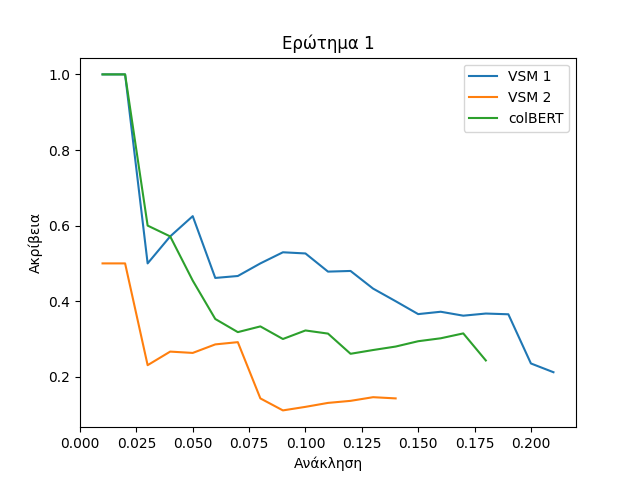
\includegraphics[scale=0.5]{1}
        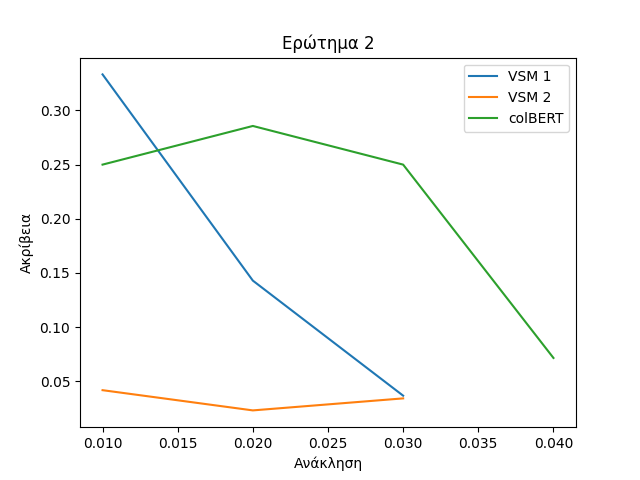
\includegraphics[scale=0.5]{2}
        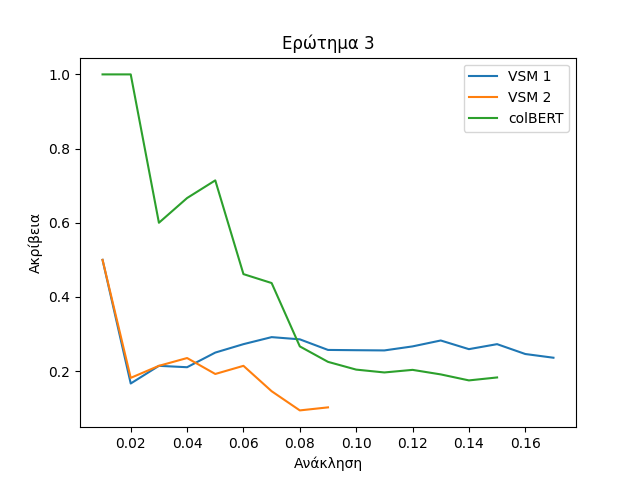
\includegraphics[scale=0.5]{3}
        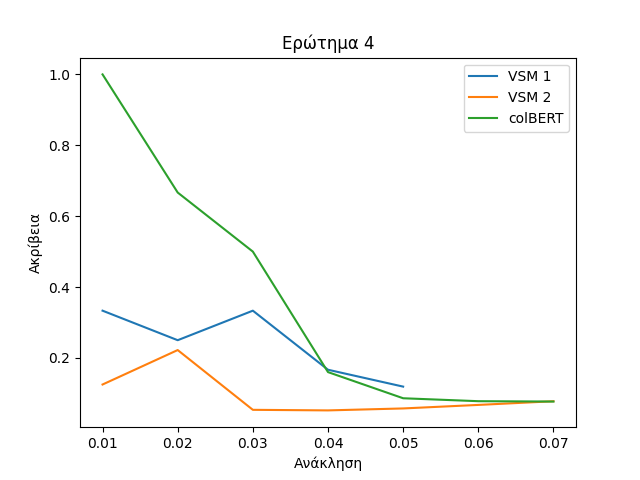
\includegraphics[scale=0.5]{4}
        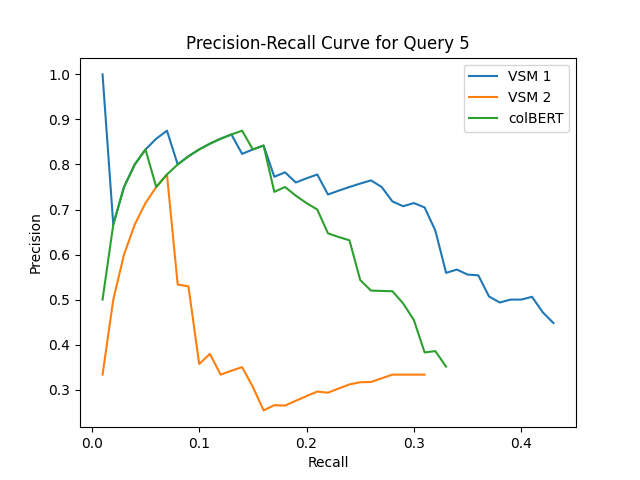
\includegraphics[scale=0.5]{5}
        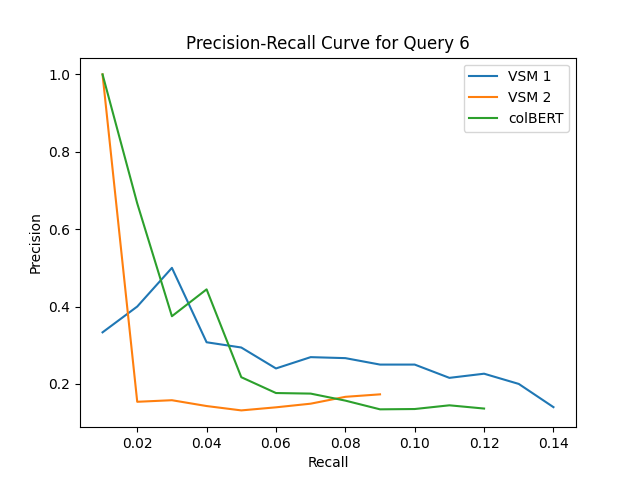
\includegraphics[scale=0.5]{6}
        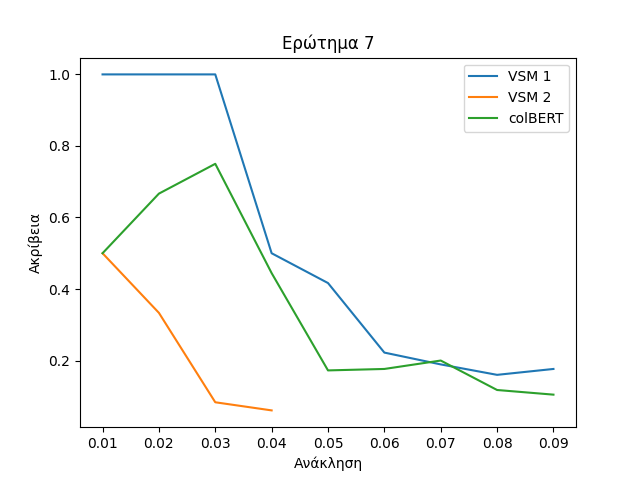
\includegraphics[scale=0.5]{7}
        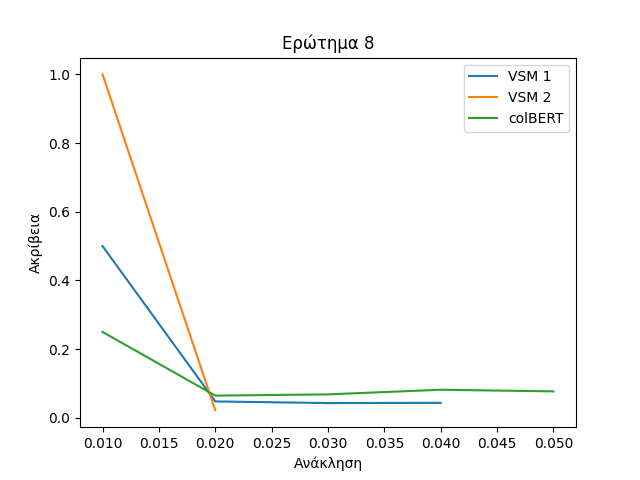
\includegraphics[scale=0.5]{8}
        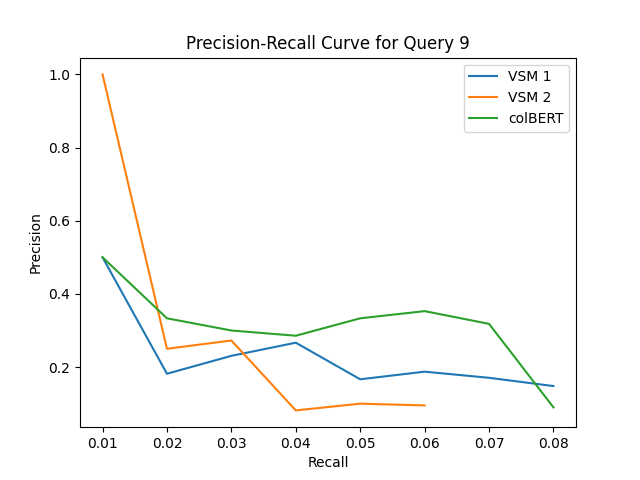
\includegraphics[scale=0.5]{9}
        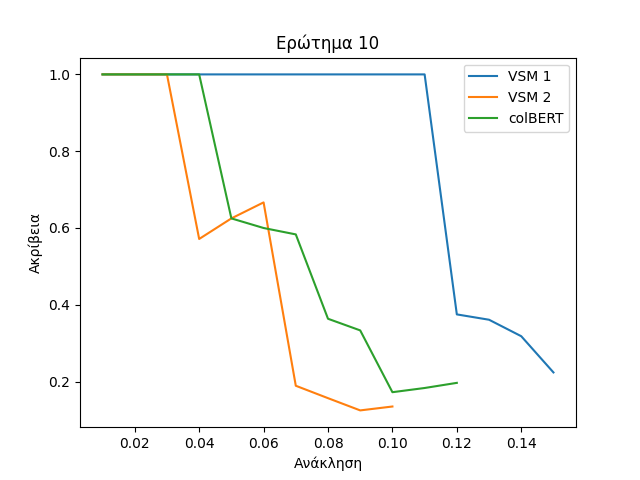
\includegraphics[scale=0.5]{10}
        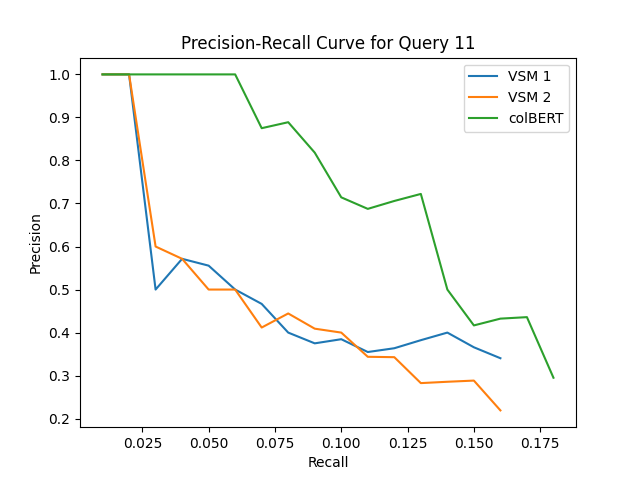
\includegraphics[scale=0.5]{11}
        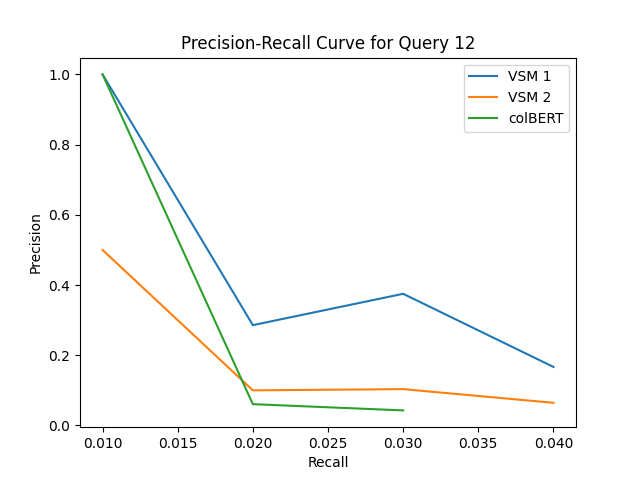
\includegraphics[scale=0.5]{12}
        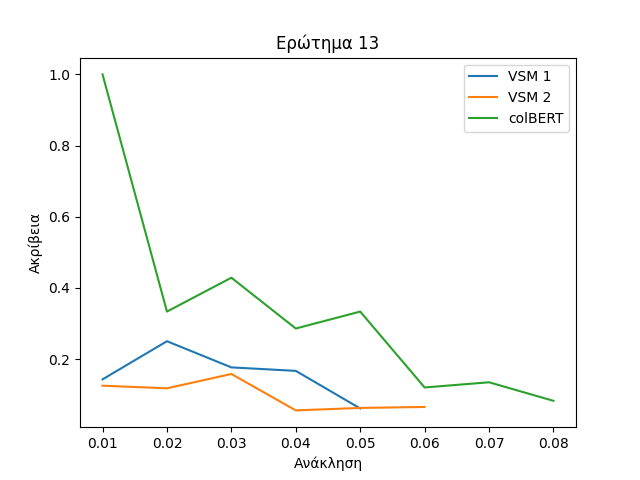
\includegraphics[scale=0.5]{13}
        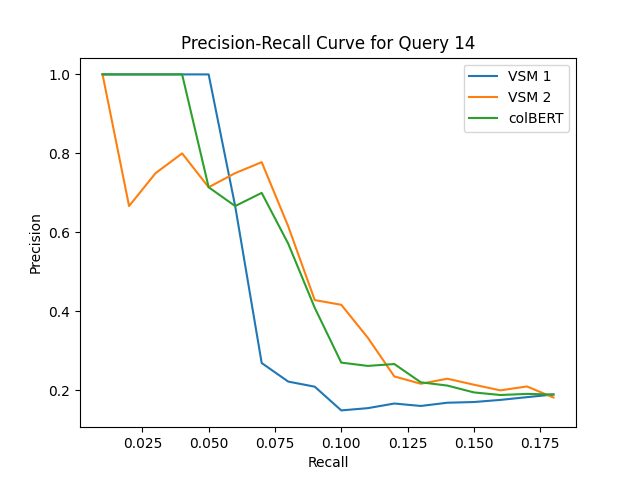
\includegraphics[scale=0.5]{14}
        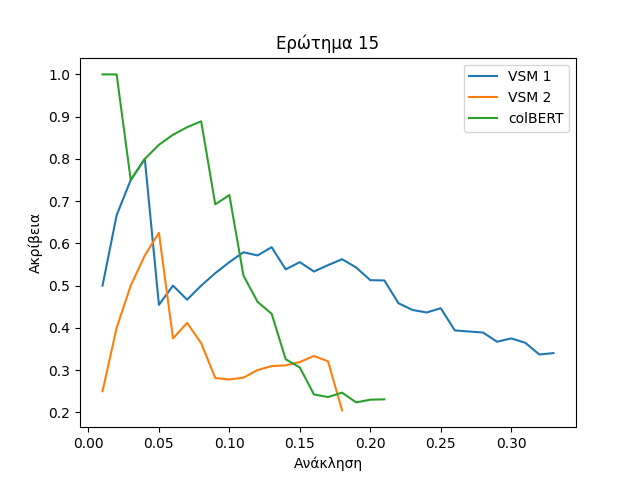
\includegraphics[scale=0.5]{15}
        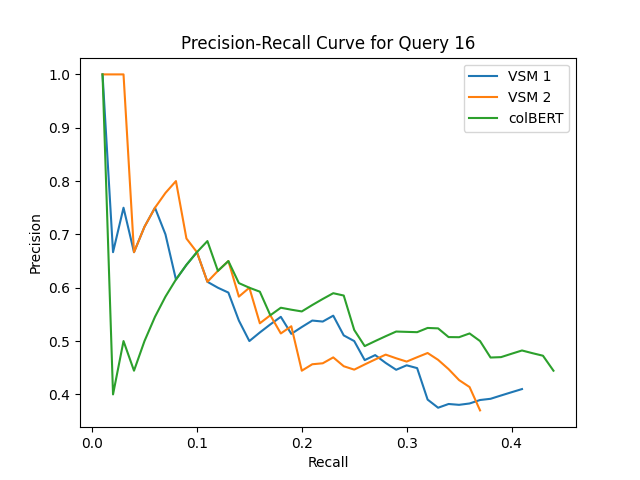
\includegraphics[scale=0.5]{16}
        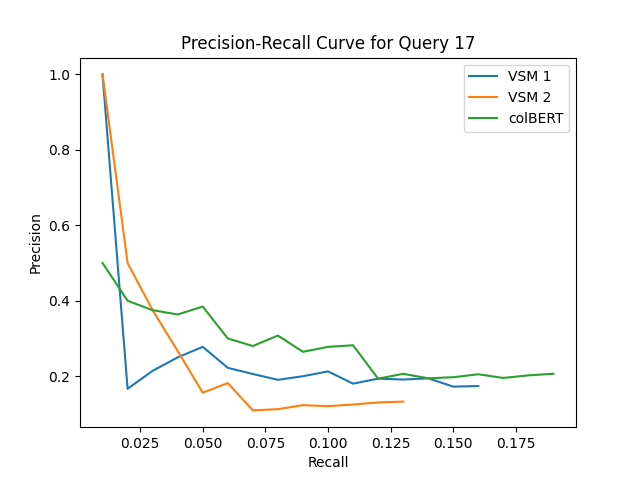
\includegraphics[scale=0.5]{17}
        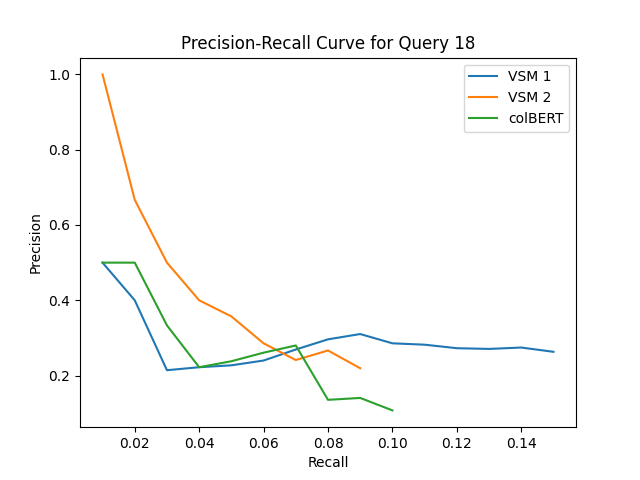
\includegraphics[scale=0.5]{18}
        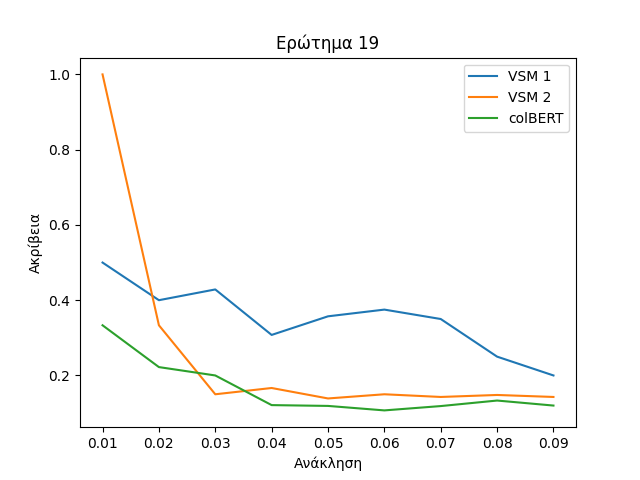
\includegraphics[scale=0.5]{19}
    \end{multicols}


    \chapter{ΠΑΡΑΡΤΗΜΑ}
    \subsection{\texttt{tools.py}}
\begin{lstlisting}[language=Python]
import json
import os


def get_docs():
    docs_directory = 'Collection/docs'
    filename_list = [file for file in os.listdir(docs_directory)]

    doc_tuples_list = []

    for filename in filename_list:
        with open(os.path.join(docs_directory, filename), 'r') as doc_file:
            doc = doc_file.readlines()
            doc = [word.strip() for word in doc]
            doc_tuple = (filename, doc)  # (DocID, <doc>)
            doc_tuples_list.append(doc_tuple)

    return doc_tuples_list


def get_queries():
    filename = 'Collection/Queries_20'

    with open(filename, 'r') as queries_file:
        queries = queries_file.readlines()

    return queries


def get_json_file(json_file):
    with open(json_file, 'r') as file:
        json_data = json.load(file)

    return json_data


def get_relevant():
    relevant_docs = {}
    with open('Collection/Relevant_20', 'r') as file:
        for i, line in enumerate(file):
            relevant_docs[i] = [int(item) for item in line.split()]

    return relevant_docs
\end{lstlisting}


\subsection{\texttt{preprocessing.py}}
\begin{lstlisting}[language=Python]
from nltk.corpus import stopwords
from nltk.stem.porter import PorterStemmer
import tools


def preprocess_collection():
    doc_tuples_list = tools.get_docs()

    stop_words = set(stopwords.words('english'))
    stemmer = PorterStemmer()

    stripped_docs = []

    for doc_tuple in doc_tuples_list:
        stripped_doc = [stemmer.stem(word.lower()) for word in doc_tuple[1] if word.lower() not in stop_words]
        stripped_doc_tuple = (doc_tuple[0], stripped_doc)  # (DocID, <stripped_doc>)
        stripped_docs.append(stripped_doc_tuple)

    return stripped_docs


def preprocess_queries():
    queries = tools.get_queries()

    stop_words = set(stopwords.words('english'))
    stemmer = PorterStemmer()

    stripped_queries = []

    for query in queries:
        stripped_query = [stemmer.stem(word.lower()) for word in query.split() if word.lower() not in stop_words]
        stripped_queries.append(stripped_query)

    stripped_queries_new = []
    for query in stripped_queries:
        query = list(set(query))
        stripped_queries_new.append(query)

    return stripped_queries_new
\end{lstlisting}


\subsection{\texttt{inverted\_index.py}}
\begin{lstlisting}[language=Python]
def create_inverted_index(stripped_docs_tuples):
    inverted_index = {}

    for doc_tuple in stripped_docs_tuples:
        for term in doc_tuple[1]:
            if term not in inverted_index:
                inverted_index[term] = set()
            inverted_index[term].add((doc_tuple[0], doc_tuple[1].count(term)))

    return inverted_index
\end{lstlisting}


\subsection{\texttt{vector\_space\_model.py}}
\begin{lstlisting}[language=Python]
import math
import numpy as np
from numpy.linalg import norm

def idf1(N, n):
    return math.log(N / n)

def idf2(N, n):
    return math.log(N - n / n)

def get_value(item):
    return item[1]


def vsm(doc_collection, query, inverted_index, model_type):
    query_tfidfs = {}
    doc_tfidfs = {}
    for doc in doc_collection:
        doc_tfidfs[doc[0]] = []  # Αρχικοποίηση λεξικού tf-idf τιμών με άδειες λίστες για κάθε έγγραφο

    # Υπολογισμός TF όρων για το ερώτημα:
    query_tfs = {}
    for term in query:
        query_tfs[term] = query.count(term)

    # Υπολογισμός TF-IDF τιμών. Διατρέχουμε κάθε όρο από το ερώτημα...
    for term in query:
        docs_containing_term = set()

        # Αν ο όρος του ερωτήματος υπάρχει στο ανεστραμμένο ευρετήριο, υπολογίζουμε την IDF τιμή του.
        if term in inverted_index:
            if model_type == "1":
                idf = idf1(len(doc_collection), len(inverted_index[term]))
            elif model_type == "2":
                idf = idf2(len(doc_collection), len(inverted_index[term]))

            # και την TF-IDF τιμή, δηλαδή το ΒΑΡΟΣ ΟΡΟΥ ΕΡΩΤΗΜΑΤΟΣ
            if model_type == "1":
                query_tfidfs[term] = (0.5 + 0.5 * (query_tfs[term] / max(query_tfs.values()))) * idf
            elif model_type == "2":
                query_tfidfs[term] = idf

            # Υπολογισμός TF-IDF τιμών για τα έγγραφα:
            for item in inverted_index[term]:
                docs_containing_term.add(item[0])
                # το docs_containing_term περιέχει τα έγγραφα που περιέχουν τον συγκεκριμένο όρο.

            # διατρέχουμε τα έγγραφα του docs_containing_term...
            for doc in doc_collection:
                if doc[0] in docs_containing_term:
                    # έγγραφο βρέθηκε - υπολογίζουμε TF
                    for item in inverted_index[term]:
                        if item[0] == doc[0]:
                            doc_tf = item[1]
                            break
                    # υπολογισμός TFIDF
                    if model_type == "1":
                        doc_tfidfs[doc[0]].append(doc_tf * idf1(len(doc_collection), len(inverted_index[term])))
                    elif model_type == "2":
                        doc_tfidfs[doc[0]].append(0.5 + 0.5 * (query_tfs[term] / max(query_tfs.values())))
                else:
                    # δε βρέθηκε έγγραφο, 0 στο διάνυσμα
                    doc_tfidfs[doc[0]].append(0)

    similarity = {}
    for doc in doc_tfidfs:
        similarity[doc] = np.dot(list(query_tfidfs.values()), doc_tfidfs[doc]) / (
                    norm(list(query_tfidfs.values())) * norm(doc_tfidfs[doc]))

    # μετατροπή nan τιμών σε 0
    similarity = {k: 0 if np.isnan(v) else v for k, v in similarity.items()}
    sort_similarity = sorted(similarity.items(), key=get_value)

    return sort_similarity[-100:][::-1]


def run_vsm(doc_collection, queries, inverted_index):
    results1 = []
    results2 = []

    for query in queries:
        results1.append(vsm(doc_collection, query, inverted_index, "1"))
        results2.append(vsm(doc_collection, query, inverted_index, "2"))

    return results1, results2
\end{lstlisting}


\subsection{\texttt{colBERT\_preprocessing.py}}
\begin{lstlisting}[language=Python]
import json
import tools

docs = tools.get_docs()
queries = tools.get_queries()

ColBERTqueries = {}
for i, query in enumerate(queries):
    ColBERTqueries[str(i)] = query.strip().upper()

colBERTdocs = {}
for i, doc in enumerate(docs):
    colBERTdocs[doc[0]] = doc[1]

with open("colBERT_input/colBERT_docs", "w") as filename:
    json.dump(colBERTdocs, filename)
    filename.close()

with open("colBERT_input/colBERT_queries", "w") as filename:
    json.dump(ColBERTqueries, filename)
    filename.close()
\end{lstlisting}


\subsection{\texttt{colBERT\_.ipynb}}
\noindent Εισαγωγή Βιβλιοθηκών/ColBERT
\begin{lstlisting}[language=Python]
!git -C ColBERT/ pull || git clone https://github.com/stanford-futuredata/ColBERT.git
import sys; sys.path.insert(0, 'ColBERT/')
try: # When on google Colab, let's install all dependencies with pip.
    import google.colab
    !pip install -U pip
    !pip install -e ColBERT/['faiss-gpu','torch']
except Exception:
  import sys; sys.path.insert(0, 'ColBERT/')
  try:
    from colbert import Indexer, Searcher
  except Exception:
    print("If you're running outside Colab, please make sure you install ColBERT in conda following the instructions in our README. You can also install (as above) with pip but it may install slower or less stable faiss or torch dependencies. Conda is recommended.")
    assert False
import colbert
from colbert import Indexer, Searcher
from colbert.infra import Run, RunConfig, ColBERTConfig
from colbert.data import Queries, Collection
\end{lstlisting}
Εισαγωγή αρχείων
\begin{lstlisting}[language=Python]
import json

with open('colBERT_docs', "r") as file:
  doc_list = json.load(file)

with open('colBERT_queries', "r") as file:
  query_list = json.load(file)

doc_ids = list(doc_list.keys())
doc_content = list(doc_list.values())

query_ids = list(query_list.keys())
query_content = list(query_list.values())

nbits = 2
doc_maxlen = 300
\end{lstlisting}
Δημιουργία Indexer - Searcher
\begin{lstlisting}[language=Python]
checkpoint = 'colbert-ir/colbertv2.0'

with Run().context(RunConfig(nranks=1, experiment='notebook')):  # nranks specifies the number of GPUs to use
    config = ColBERTConfig(doc_maxlen=doc_maxlen, nbits=nbits, kmeans_niters=20) # kmeans_niters specifies the number of iterations of k-means clustering; 4 is a good and fast default.
                                                                                # Consider larger numbers for small datasets.

    indexer = Indexer(checkpoint=checkpoint, config=config)
    indexer.index(name='index_name', collection=doc_content, overwrite=True)

with Run().context(RunConfig(experiment='notebook')):
    searcher = Searcher(index='index_name', collection=doc_content)
\end{lstlisting}

Αποτελέσματα:
\begin{lstlisting}[language=Python]
results = []
for query in query_content:
  result = searcher.search(query, k=100)

  passages = []
  for passage_id, passage_rank, passage_score in zip(*result):
      passages.append(int(doc_ids[passage_id]))
  results.append(passages)
print(results)

from google.colab import files
import json

with open("colBERT_output.json", "w") as file:
  json.dump(results, file)

files.download("colBERT_output.json")
\end{lstlisting}


\subsection{\texttt{evaluation\_metrics.py}}
\begin{lstlisting}[language=Python]
import tools
import matplotlib.pyplot as plt
import numpy as np


def recall_precision(results, model):
    # results: λίστα (όλων των queries) που περιλαμβάνει λίστες με τα πιο σχετικά έγγραφα, όπως υπολογίστηκαν από το cosine similarity
    relevant_docs = tools.get_relevant()
    # relevant_docs: dictionary με τις τιμές των πραγματικά σχετικών εγγράφων του Relevent_20

    recall_precision_values = []

    if model == "vsm":
        # Το results περιλαμβάνει συγκεντρωτικά όλα τα αποτελέσματα για κάθε query. Διατρέχουμε το κάθε query μεμονομένα...
        for i, results_query in enumerate(results):
            precision = []
            recall = []
            truly_relevant_docs = 0
            # διατρέχουμε τα πιο σχετικά έγγραφα για το συγκεκριμένο query...
            for j, doc in enumerate(results[i]):
                if type(doc) == tuple:
                    current_doc = int(doc[0])
                    if current_doc in relevant_docs[i]:
                        truly_relevant_docs += 1

                        recall.append(truly_relevant_docs / len(results_query))
                        precision.append(truly_relevant_docs / (j + 1))

            recall_precision_values.append((recall, precision))

    if model == "colBERT":
        for i, results_query in enumerate(results):
            precision = []
            recall = []
            truly_relevant_docs = 0
            for j, doc in enumerate(results[i]):
                if doc in relevant_docs[i]:
                    truly_relevant_docs += 1

                    recall.append(truly_relevant_docs / len(results_query))
                    precision.append(truly_relevant_docs / (j + 1))

            recall_precision_values.append((recall, precision))

    return recall_precision_values


def mean_average_precision(recall_precision_values):
    average_precision_list = []
    for i in range(len(recall_precision_values)):
        recalls, precisions = recall_precision_values[i]
        average_precision = 0

    for j in range(1, len(recalls)):
        average_precision += (recalls[j] - recalls[j - 1]) * precisions[j]
        average_precision_list.append(average_precision)

    return np.mean(average_precision_list)


def run_metrics(vsm1_results, vsm2_results):
    colBERT_results = tools.get_json_file("colBERT_output.json")

    recall_precision_vsm1 = recall_precision(vsm1_results, "vsm")
    recall_precision_vsm2 = recall_precision(vsm2_results, "vsm")
    recall_precision_colBERT = recall_precision(colBERT_results, "colBERT")

    map_vm1 = mean_average_precision(recall_precision_vsm1)
    map_vm2 = mean_average_precision(recall_precision_vsm2)
    map_colBERT = mean_average_precision(recall_precision_colBERT)

    print("vm1", map_vm1)
    print("vm2", map_vm2)
    print("colBERT", map_colBERT)

    for i in range(len(recall_precision_vsm1)):
        plt.figure()
        plt.plot(recall_precision_vsm1[i][0], recall_precision_vsm1[i][1], label="VSM 1")
        plt.plot(recall_precision_vsm2[i][0], recall_precision_vsm2[i][1], label="VSM 2")
        plt.plot(recall_precision_colBERT[i][0], recall_precision_colBERT[i][1], label="colBERT")
        plt.xlabel('Ανάκληση')
        plt.ylabel('Ακρίβεια')
        plt.title(f'Ερώτημα {i + 1}')
        plt.legend(loc='upper right')
        plt.savefig('Precision_Recall_Curve/' + str(i + 1) + '.png')
\end{lstlisting}


\subsection{\texttt{main.py}}
\begin{lstlisting}[language=Python]
import inverted_index as ii
import vector_space_model as vsm
import preprocessing as prep
import evaluation_metrics as metrics

def main_app():
    doc_collection = prep.preprocess_collection()   # stripped_docs
    queries = prep.preprocess_queries()     # stripped_queries

    inverted_index = ii.create_inverted_index(doc_collection)
    results1, results2 = vsm.run_vsm(doc_collection, queries, inverted_index)

    metrics.run_metrics(results1, results2)


if __name__ == '__main__':
    main_app()

\end{lstlisting}

\end{document}
